\chapter{Family of Hidden Markov Models}
\index{Family of Hidden Markov Models@\emph{Family of Hidden Markov Models}}\label{hmmfamily}

In this chapter I present a new statistical model for representing an MSA called the Family of Hidden Markov Models (fHMM).  In Section~\ref{hmmfamily:model}, I describe the fHMM and how to build the fHMM.  In Section~\ref{hmmfamily:alignment}, I describe an algorithm for sequence alignment using the fHMM.  

\section{Family of HMM}\label{hmmfamily:model}
The fHMM is a statistical model for representing an MSA using a collection of HMMs.  The model was originally developed in SEPP~\cite{Mirarab2012} for the problem of phylogenetic placement.  During our SEPP study, we realized that the utility of fHMM extends beyond phylogenetic placement.  More specifically, the fHMM can used as a replacement of an HMM for sequence alignment.  

\paragraph{Building an fHMM.}  The basic outline for building an fHMM is to divide the input MSA into subsets of closely related sequences.  HMMs are computed on the individual subsets, and these HMMs make up the fHMM.  I now provide more details on this process.  

The necessary inputs for building the fHMM are an MSA (called the ``backbone alignment''), a tree on the sequences in the MSA (called the ``backbone tree''), and a maximum alignment decomposition size parameter $m_a$.  The first step is to use the backbone tree to decompose the alignment into subsets of size at most $m_a$.  We do this through a recursive decomposition technique called the ``centroid edge decomposition''~\cite{Liu2012}.

From the backbone tree, we select the centroid edge $e$ (one whose removal separates the leaf set into approximately two equally sized subsets).  We remove $e$ from the backbone tree to produce two subtrees.  For each subtree with more than $m_a$ leaves, we recursively repeat this decomposition until all the subtrees produced by this decomposition have at most $m_a$ leaves.  

Figure~\ref{hmmfamily:decomp} shows this process explicitly.  The backbone tree in the figure has 11 taxa, and $m_a$ is set to 3.  In step 1, the centroid edge (colored red) is removed.  This splits the tree into subtrees contains 5 taxa and 6 taxa.  In step 2, each of these subtrees are further subdivided into trees of sizes 2, 2, 3, and 4.  In step 3, one final centroid decomposition divides the subtree of size 4 into two subtrees of size 2 and 2.  Step 4 shows the final result of this decomposition; the original backbone tree has now been decomposed into 5 subtrees, all with at most 3 leaves.

\begin{figure}[htbp]
\centering
{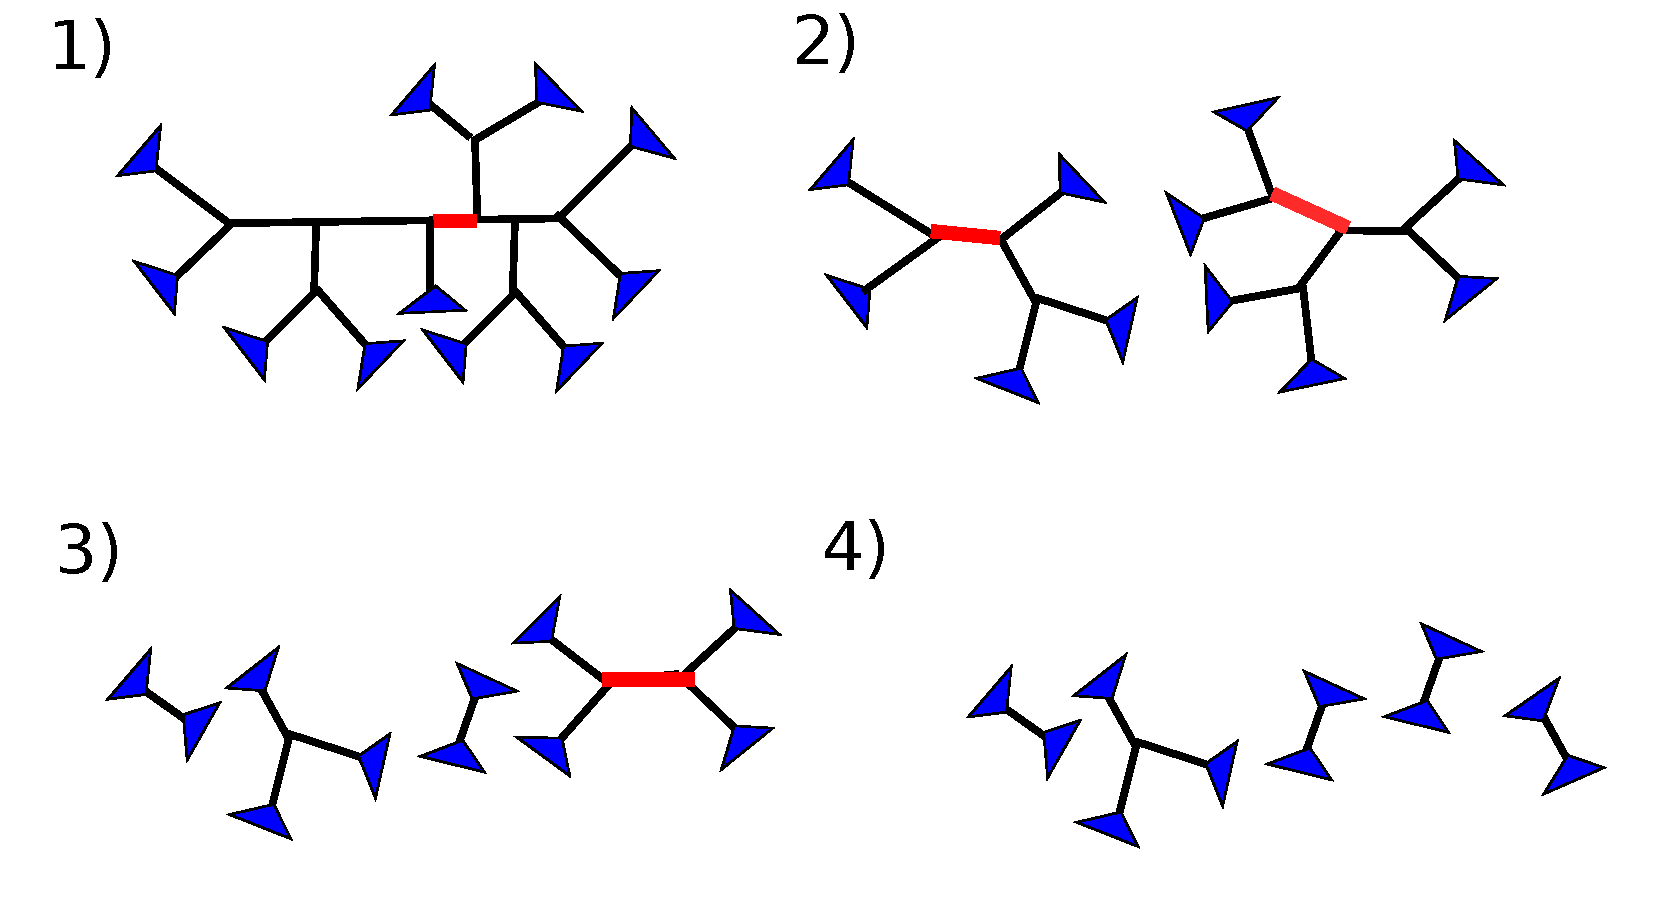
\includegraphics[width=.750\textwidth]{hmmfamily/decomposition_2}}
\caption[Example of centroid decomposition.]{Example of centroid decomposition.  The centroid edge (colored red) partitions the tree into roughly two equally sized subtrees.  This edge is removed, and two subtrees are created.  This process is recursively repeated on the subtrees until all subtrees contain at most as many sequences as the maximum decomposition size $m_a$.  In this example, $m_a=3$.} 
\label{hmmfamily:decomp}
\end{figure}

For a given subtree, we compute the alignment induced on the sequences present in the subtree's leaf set.  This is done by selecting the alignment of the sequences from the backbone alignment.  Note that the induced alignment may contain some sites that are fully gapped; these sites are removed from the subalignment.  The HMM is then computed on the subalignment using HMMBUILD~\cite{hmmer} (see Fig.~\ref{hmmfamily:hmmbuild}).

\begin{figure}[htbp]
\centering
{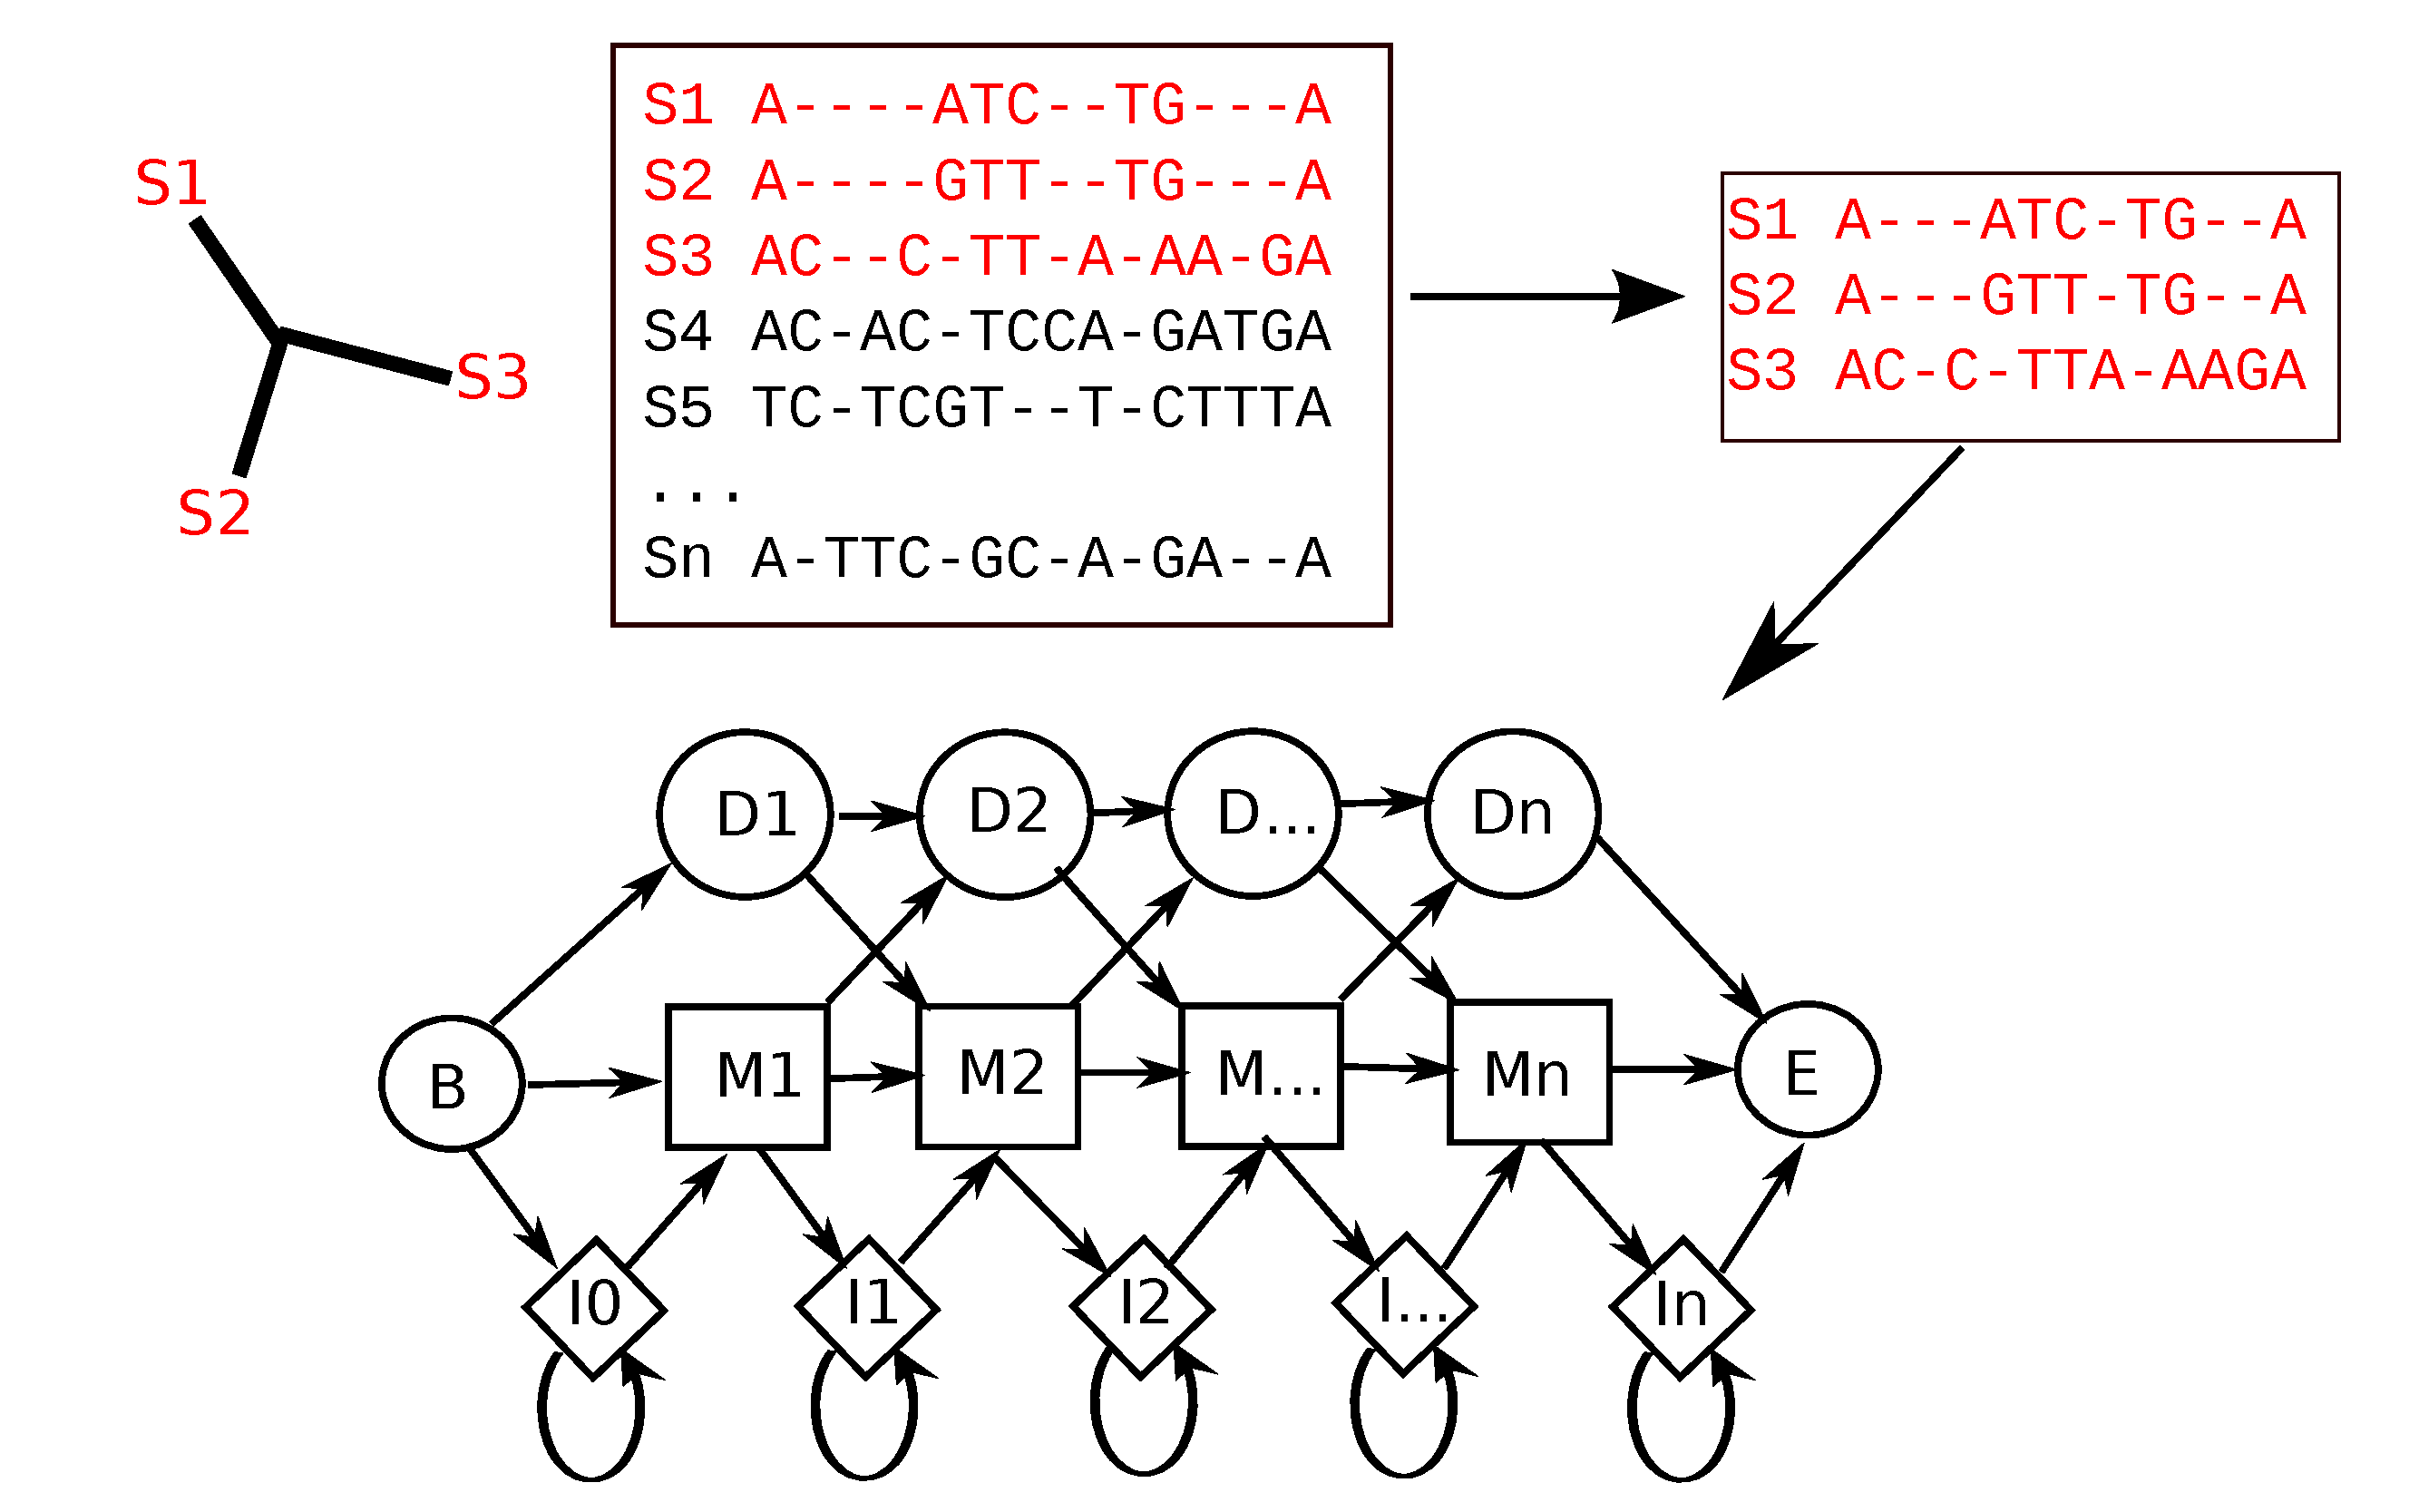
\includegraphics[width=.750\textwidth]{hmmfamily/build_hmm}}
\caption[Building an HMM.]{Example of building an HMM.  Each of the final subtrees produced by the decomposition step defines a subalignment.  For a given subtree, an induced alignment is created by taking the alignment of the sequences that are in the leaf set of the tree.  Next, an HMM is computed on the induced alignment using HMMBUILD.} 
\label{hmmfamily:hmmbuild}
\end{figure}

\section{fHMM alignment algorithm}\label{hmmfamily:alignment}
For a given query sequence $q$, it is scored against each of the HMMs using HMMSEARCH~\cite{hmmer}, which reports a HMMER ``bit score'', a measure of the quality of the match between the query sequence $q$ and the HMM (see Fig.~\ref{hmmfamily:align}).  The HMM that yields the best bit score is selected, and an extended subalignment is produced by inserting $q$ into the subalignment using HMMALIGN.  

(i.e., characters in the query sequence that are not homologous to any characters in the backbone alignment) 

\begin{figure}[htbp]
\centering
{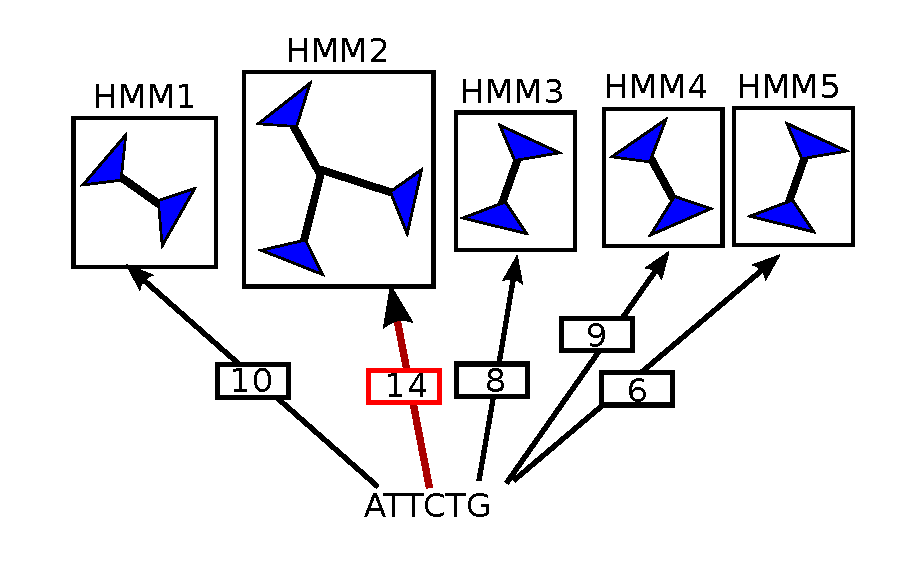
\includegraphics[width=1.0\textwidth]{hmmfamily/search_2.pdf}}
\caption[Example of alignment using HMM families.]{Example of aligning a query sequence using the families of HMMs.  The query sequence is scored against a collection of HMMs.  The HMM that yields the best bit score, HMM-2 in this case, is selected and the query sequence is aligned to that HMM.} 
\label{hmmfamily:align}
\end{figure}

Finally, we extend $q$'s alignment to the entire backbone alignment (see Fig.~\ref{hmmfamily:trans}).  This step is performed through transitivity.  We can map the sites in the subalignment back to the original backbone alignment, and thus, any sequence that is aligned to the subalignment can easily be aligned to the backbone alignment by using this mapping.  Note that insertion columns generated by the alignment of the query sequence result in insertion columns being added to the backbone alignment.

\begin{figure}[htbp]
\centering
{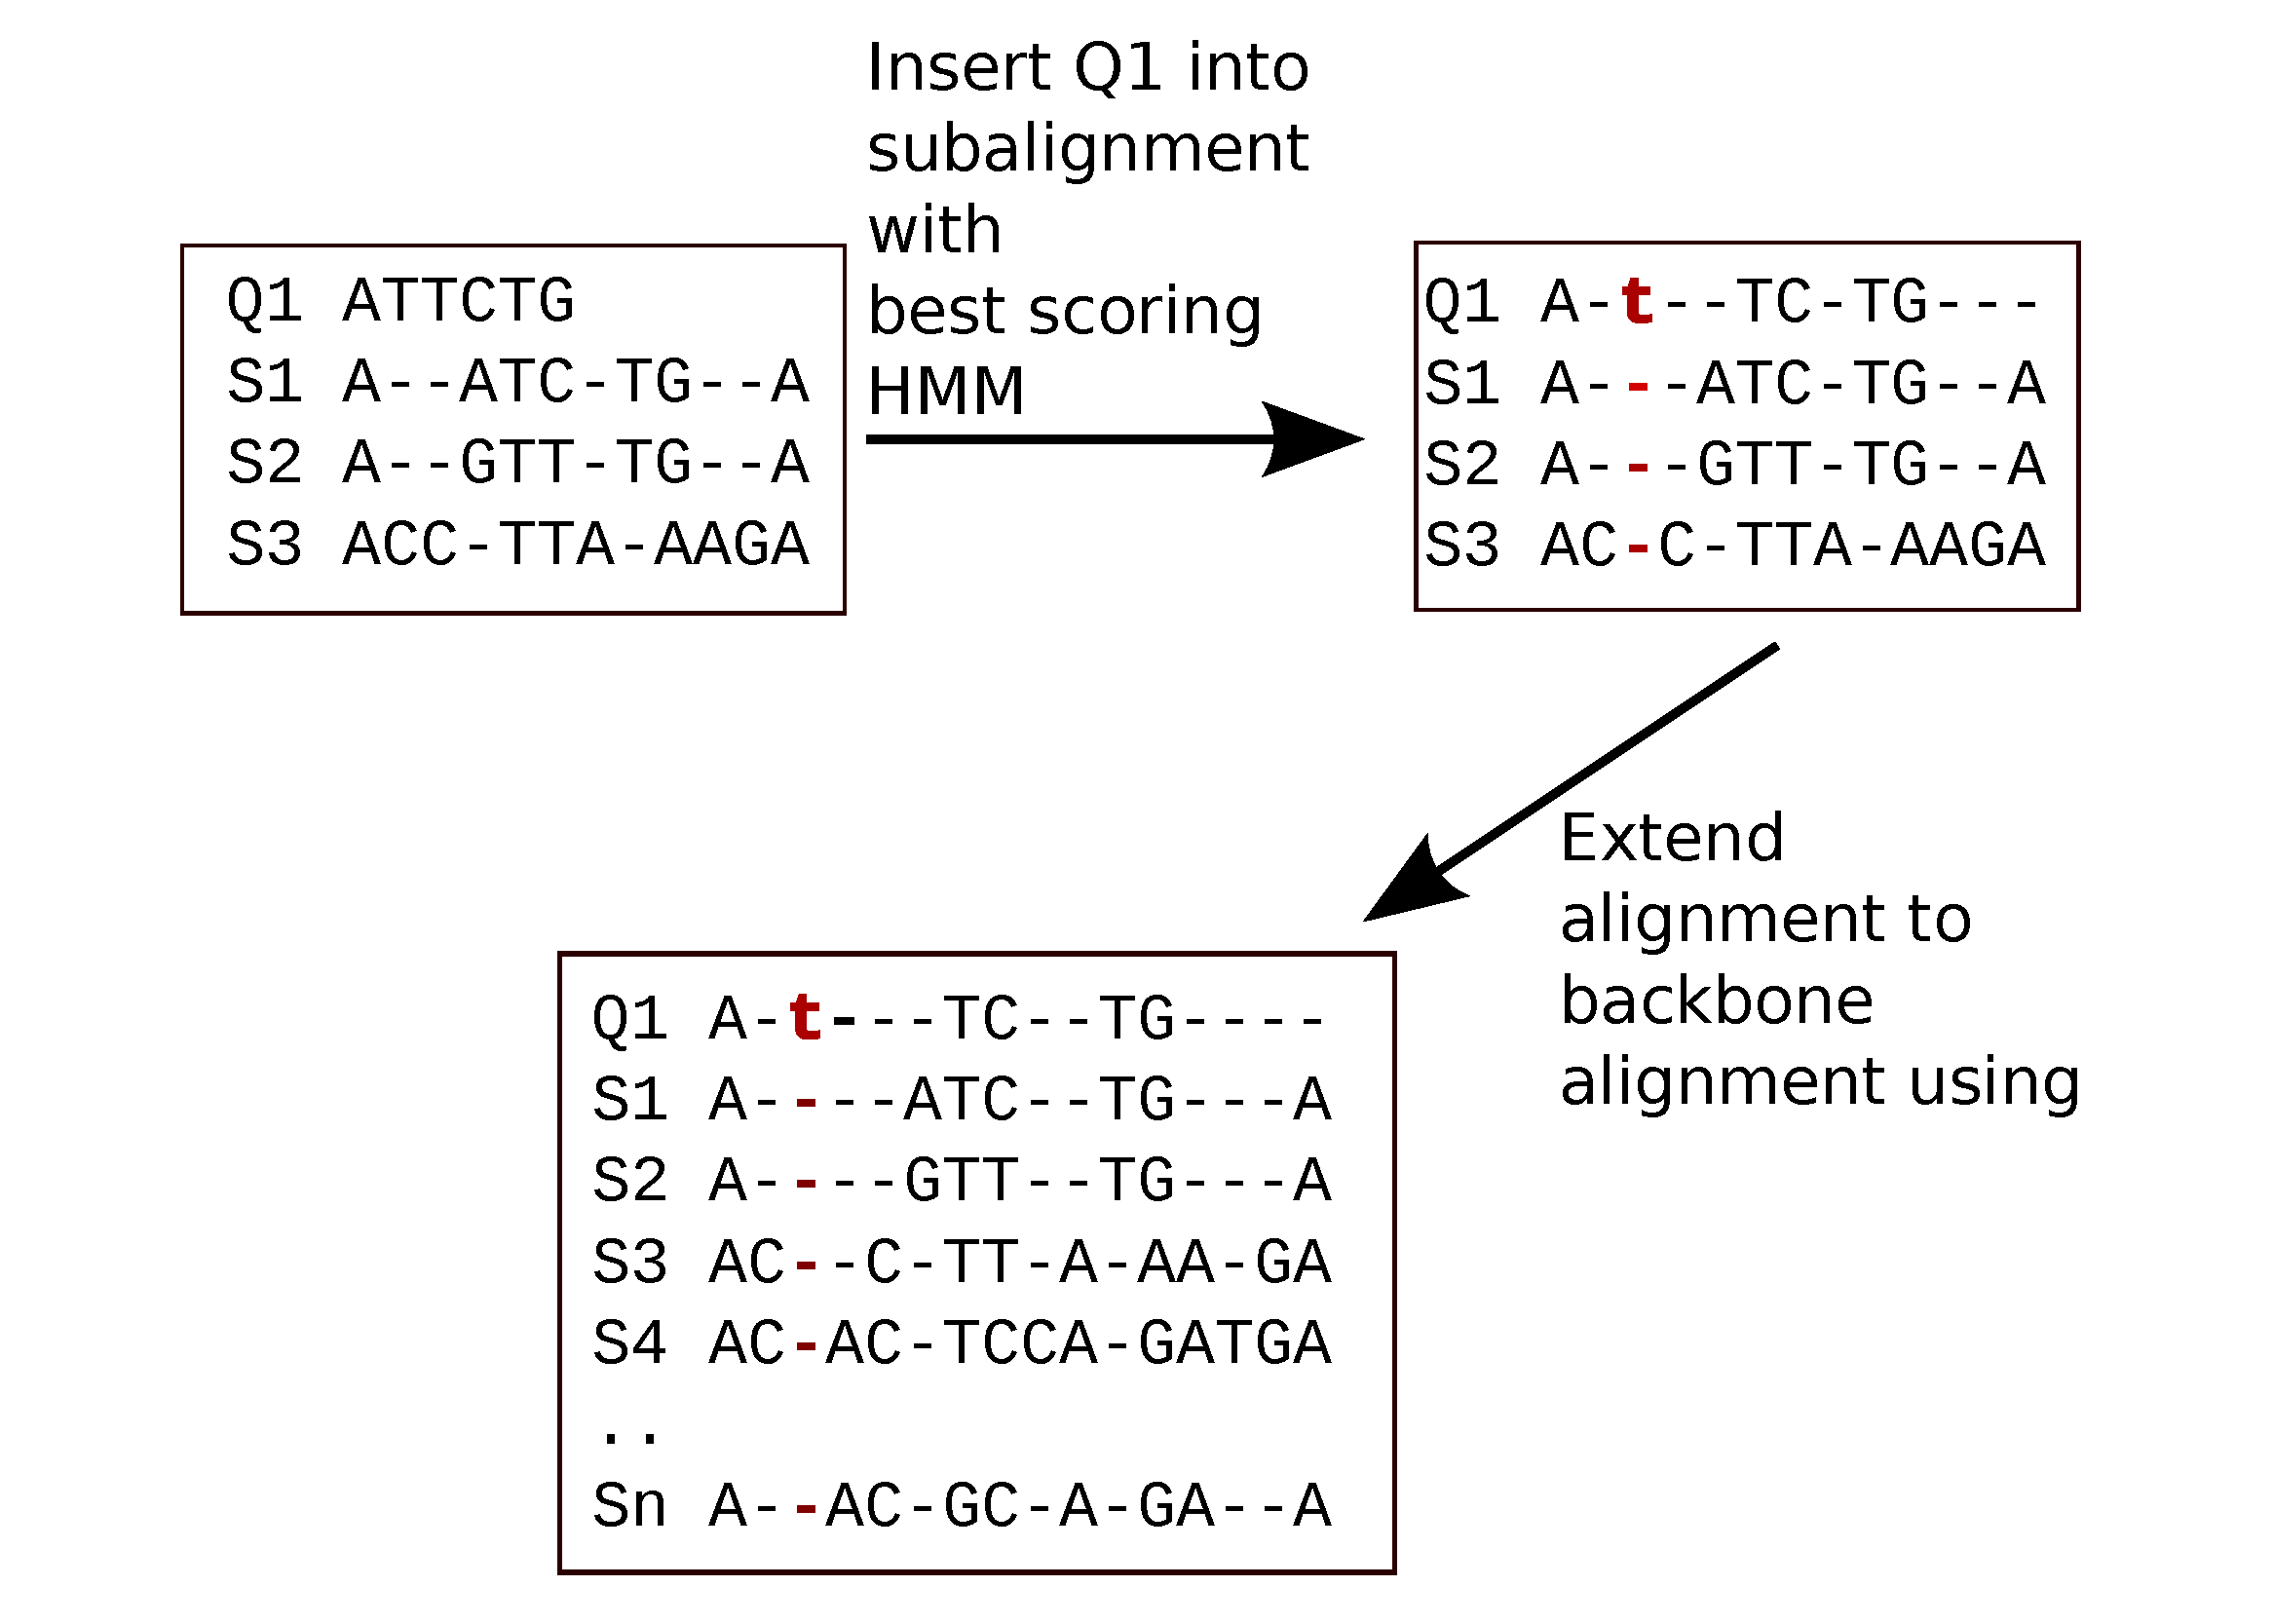
\includegraphics[width=1.0\textwidth]{hmmfamily/insertion}}
\caption[Example of alignment of query sequence through transitivity.]{Example of extending the alignment of query sequence to the full backbone alignment through transitivity.  We know how the sites of the subalignment map back to the original backbone alignment, so we use this information to map the alignment of the query sequence to the alignment on the entire backbone alignment.  Note that insertion columns (shown in red) are also inserted into the backbone alignment.} 
%\textbf{NAM: number columns in subalignment/backbone alignment to make mapping more explicit}
\label{hmmfamily:trans}
\end{figure}


In the special case where a query sequence resulted in no scores against any of the HMMs (i.e., HMMSEARCH reports the sequence as non-homologous to all HMMs), the query sequence is omitted from the final alignment.  

Over the next three chapters, I show how to apply the fHMM to phylogenetic placement, taxonomic profiling and identification, and ultra-large alignment estimation.


